\documentclass[conference]{IEEEtran}
\usepackage{graphicx}
\usepackage{booktabs}
\usepackage{url}
\usepackage{amsmath}
\usepackage{multirow}
\usepackage{xeCJK}
\setCJKmainfont{SimSun}
\title{Performance Evaluation of Machine Learning Algorithms for Encrypted Proxy Traffic Identification}
\author{\IEEEauthorblockN{ZhangXiaoyuan (张校源)}\IEEEauthorblockA{Independent Researcher\\Email: silenceyuan2018@gmail.com\\ORCID: 0009-0006-6147-9256}}
\begin{document}\sloppy
\maketitle
\begin{abstract}
Encrypted proxy traffic is difficult to distinguish from other encrypted network workloads because payload inspection is unavailable. This paper reports two separate classification studies rather than a four-class proxy benchmark. JA4Tor uses five source labels; MineShark uses three mining-trace labels. Logistic Regression and native HistGradientBoosting are added as baselines, with repeated uncertainty, per-class metrics, confusion matrices, permutation importance, timing, and model sizes. XGBoost was also run on JA4Tor: 92.08% accuracy, 92.08% macro recall, 92.24% macro F1, 8.46 s fit time, 0.10 s prediction time, and a 1.77 MB serialized pipeline. On the original JA4Tor evaluation, RF reaches 92.12\% accuracy; a capture-disjoint three-class MineShark mining-trace split gives 97.27\% with SVM. Under a workload-shift experiment from NBMiner training captures to XMRig test captures, performance drops to 46.66\% for SVM, showing that source and workload dependence must be reported. We provide feature-importance analysis, an auditable data split, figures, scripts, and metadata for reproduction.
\end{abstract}
\begin{IEEEkeywords}
encrypted traffic, proxy detection, machine learning, network flows, reproducibility
\end{IEEEkeywords}

\section{Introduction}
Encrypted tunnels protect content but also limit conventional payload-based inspection. Statistical flow features offer a practical alternative for traffic classification, yet reported accuracy can be inflated by random row splits, duplicated captures, or ambiguous labels. This study focuses on an auditable baseline for encrypted proxy traffic identification and explicitly separates task-specific performance from capture-disjoint and workload-shift evaluation.

\section{Data Sources and Label Audit}
The experiments use two public sources and do not validate a Shadowsocks/VLESS/Trojan/ordinary-HTTPS four-class taxonomy. JA4Tor has no VLESS class and NonTor is not per-flow HTTPS ground truth; MineShark has ShadowsocksR and VMess labels, no VLESS, and no ordinary-HTTPS class. JA4Tor provides labeled flow records for Tor and non-Tor traffic. Its NonTor label is retained as provided and is not reinterpreted as ordinary HTTPS. MineShark contains labeled cryptocurrency-mining and proxy-related captures. In particular, the dataset label \texttt{ssr} denotes ShadowsocksR, while \texttt{v2ray} denotes VMess. The available public labels do not constitute a complete four-class benchmark covering Shadowsocks, VLESS, Trojan, and ordinary HTTPS; therefore, no four-class accuracy is claimed here.


The official ISCXVPN2016 artifact provides OpenVPN/non-VPN and application labels, which do not establish Shadowsocks, VLESS, or Trojan labels~\cite{gil}. We therefore use documented artifacts from NESTTOR/JA4Tor and MineShark~\cite{nesttor,mineshark}; their experiments are not pooled. JA4Tor comprises NonTor, Tor, Tor-over-Shadowsocks, Tor-over-Trojan, and Tor-over-VMess. Training contains 20,000 flows (4,000 per class), the primary test contains 5,000 (1,000 per class), and the second file contains 5,024. The public files lack complete row-to-capture provenance, preventing independent verification of capture-disjointness. The second test file is used as supplied; its acquisition domain is not inferred.

MineShark contributes 103 ShadowsocksR, 41 Trojan, and 64 VMess capture-derived records, yielding 12,401 eligible windows before sampling: 6,327 ShadowsocksR, 2,154 Trojan, and 3,920 VMess. The fixed seed-42 audited split assigns 72/31 ShadowsocksR, 29/12 Trojan, and 45/19 VMess capture files to train/test. Before balancing it has 8,893/3,508 windows; equal sampling leaves 4,743/1,719 (1,581/573 per class) and excludes 5,939 candidate windows. The earlier 4,743/1,719 baseline is thereby recovered from the stored candidate pool. Thus 12,401 is not the number used by one fit. Its archive MD5 is \texttt{6c64268ec35414fc9f483a7a4ed43755}. The supplied normal.pcap lacks per-flow HTTPS ground truth and is not relabeled as ordinary HTTPS. Capture files are divided approximately 70/30 within each class before balanced window sampling. IPs, ports, pool names, and acquisition dates are excluded from classifier inputs.

\section{Methodology}
JA4Tor uses 30 exact features: forward/backward packet counts and byte totals; forward/backward packet-length max, min, mean, and standard deviation; packet-length variance; Down/Up Ratio; Average Packet Size; flow duration and rates; Flow IAT mean, standard deviation, max, and min; Fwd IAT mean, standard deviation, max, and min; and Bwd IAT mean, standard deviation, max, and min. MineShark uses 20 exact window features: packet count, total bytes, duration, packet rate, frame mean/std/median/p90/min/max, IAT mean/std/median/p90/max, upstream count ratio, downstream/upstream byte ratio, upstream and downstream frame means, and direction-switch rate. Examples include mean and standard deviation of forward and backward packet lengths, maximum packet lengths, total bytes, packet counts, IAT summaries, and the down/up byte or packet ratio. Non-finite values are treated as missing and median-imputed using training data only, and numeric features are standardized for SVM and KNN.
\begin{figure*}[t]
\centering
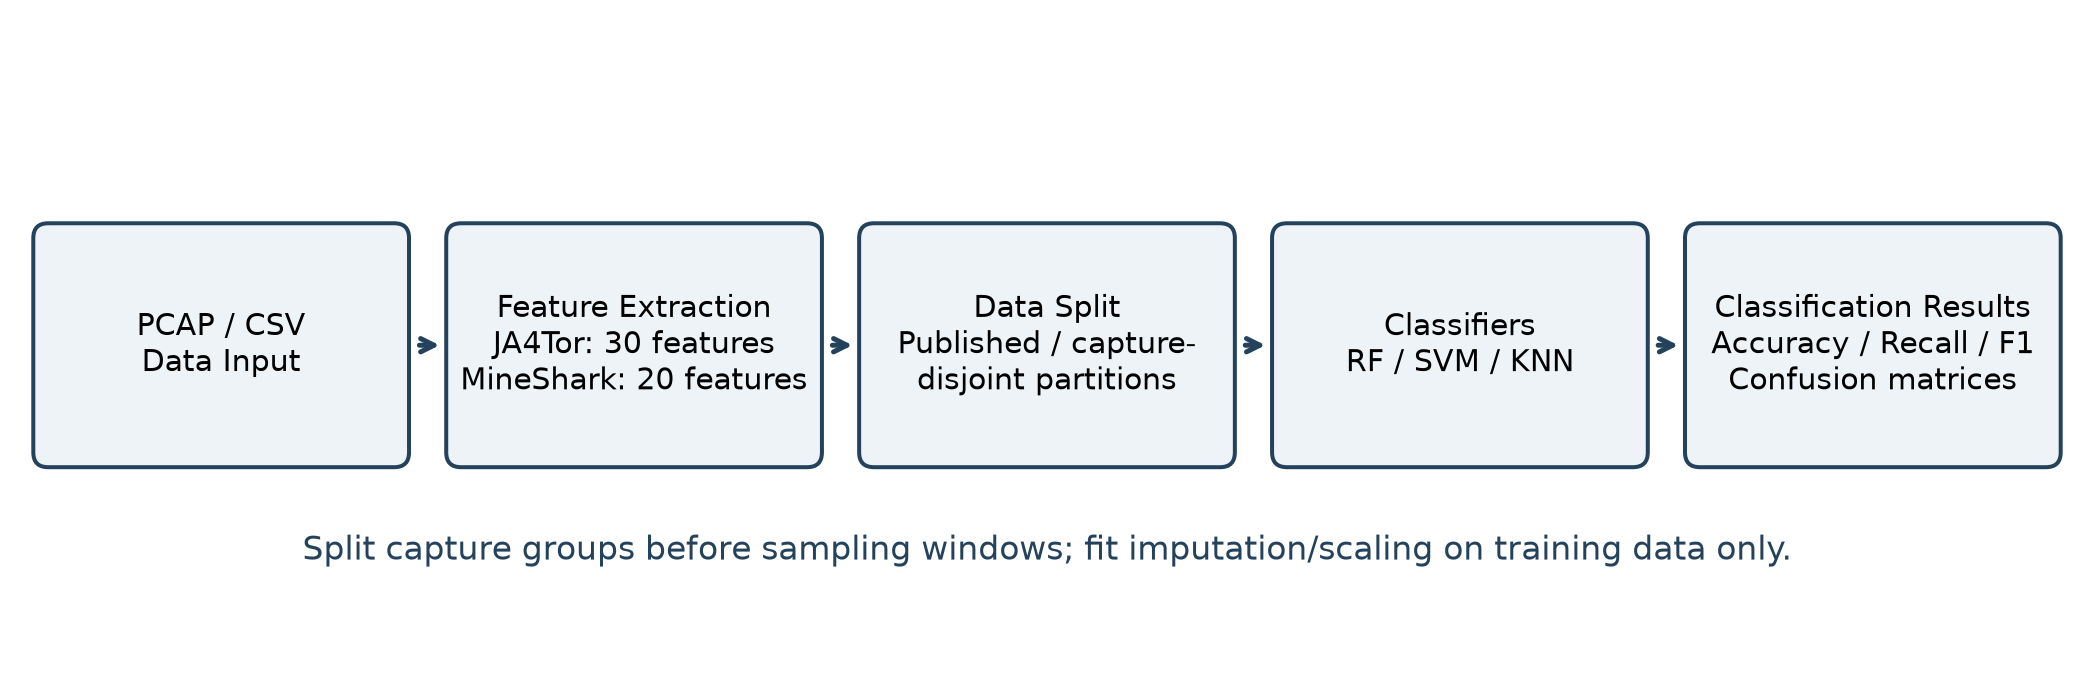
\includegraphics[width=.94\textwidth]{methodology.png}
\caption{Data processing and classifier evaluation pipeline.}
\label{fig:pipeline}
\end{figure*}
The pipeline in Fig.~\ref{fig:pipeline} reads PCAP/CSV input, extracts dataset-specific features, creates a documented split, trains RF/SVM/KNN/LogReg/HistGB/XGBoost, and reports classification metrics.


\subsection{Feature Definitions and Model Settings}
JA4Tor features are defined precisely as packet counts and byte totals in forward/backward directions; max, min, mean, and standard deviation of directional packet lengths; overall packet-length variance; Down/Up Ratio; Average Packet Size; duration and packet/byte rates; and flow, forward, and backward IAT mean, standard deviation, maximum, and minimum. The JA4Tor implementation computes duration and IAT values in microseconds and defines direction from the flow initiator. MineShark features are frame-length mean/std/median/p90/min/max, IAT mean/std/median/p90/max in milliseconds, counts and byte totals, duration, packet rate, upstream count ratio, directional byte ratio, directional frame means, and direction-switch rate. For arrival times $t_i$, $\mathrm{IAT}_i=t_i-t_{i-1}$; for byte counts $B_d,B_u$, the directional byte ratio is $B_d/\max(B_u,1)$. MineShark frame lengths include link-layer overhead and possibly oversized offloaded frames, and must not be interpreted as pure TCP payload sizes. Client direction is inferred from private addresses in preprocessing; addresses are excluded from classifier inputs.

RF uses 200 trees, square-root feature sampling, minimum leaf size 2, and random seed 42. The RBF SVM uses $C=10$ and gamma=scale; KNN uses $k=7$. Imputation and standardization are fitted on training data only. No test-set tuning is performed. Logistic Regression uses C=1 with a 2,000-iteration limit; HistGradientBoosting uses 150 iterations and 31 maximum leaves; XGBoost uses 150 histogram trees, depth 6, learning rate 0.1, and subsampling 0.9. These classifiers represent ensemble trees, nonlinear margins, and distance learning~\cite{breiman,cortes,cover,pedregosa}. Accuracy is the fraction of correct predictions; class recall is $TP/(TP+FN)$, and macro recall averages class recalls. Balanced test classes make accuracy and macro recall equal in some results.

\section{Experimental Design and Reproducibility}
For JA4Tor, we report the original test split and the separately published second test file. For MineShark, the primary split is capture-disjoint: training and test captures do not overlap. We report accuracy, macro recall, and macro F1. All saved predictions were re-evaluated independently, and the resulting metrics matched the stored CSV values. JA4Tor input hashes and the MineShark archive checksum are recorded in the repository metadata.

\section{Results}
\subsection{JA4Tor}
Table~\ref{tab:ja4tor} summarizes the baseline and second-test-file results. RF recall is 88.60\% for Tor-SS and 93.40\% for Tor-Trojan. Differences on the second file cannot be directly attributed to cross-node or cross-time generalization without capture-level provenance.
\begin{table}[t]
\caption{JA4Tor results (percent).}
\label{tab:ja4tor}
\centering
\small
\begin{tabular}{llrrr}
\toprule
Test & Model & Acc. & Recall & F1\\
\midrule
Original & RF & 92.12 & 92.12 & 92.27\\
Original & SVM & 89.72 & 89.72 & 89.90\\
Original & KNN & 88.24 & 88.24 & 88.21\\
Second & RF & 87.54 & 87.69 & 87.33\\
Second & SVM & 76.73 & 76.99 & 74.38\\
Second & KNN & 79.40 & 79.58 & 78.23\\
\bottomrule
\end{tabular}
\end{table}
\begin{figure}[t]
\centering
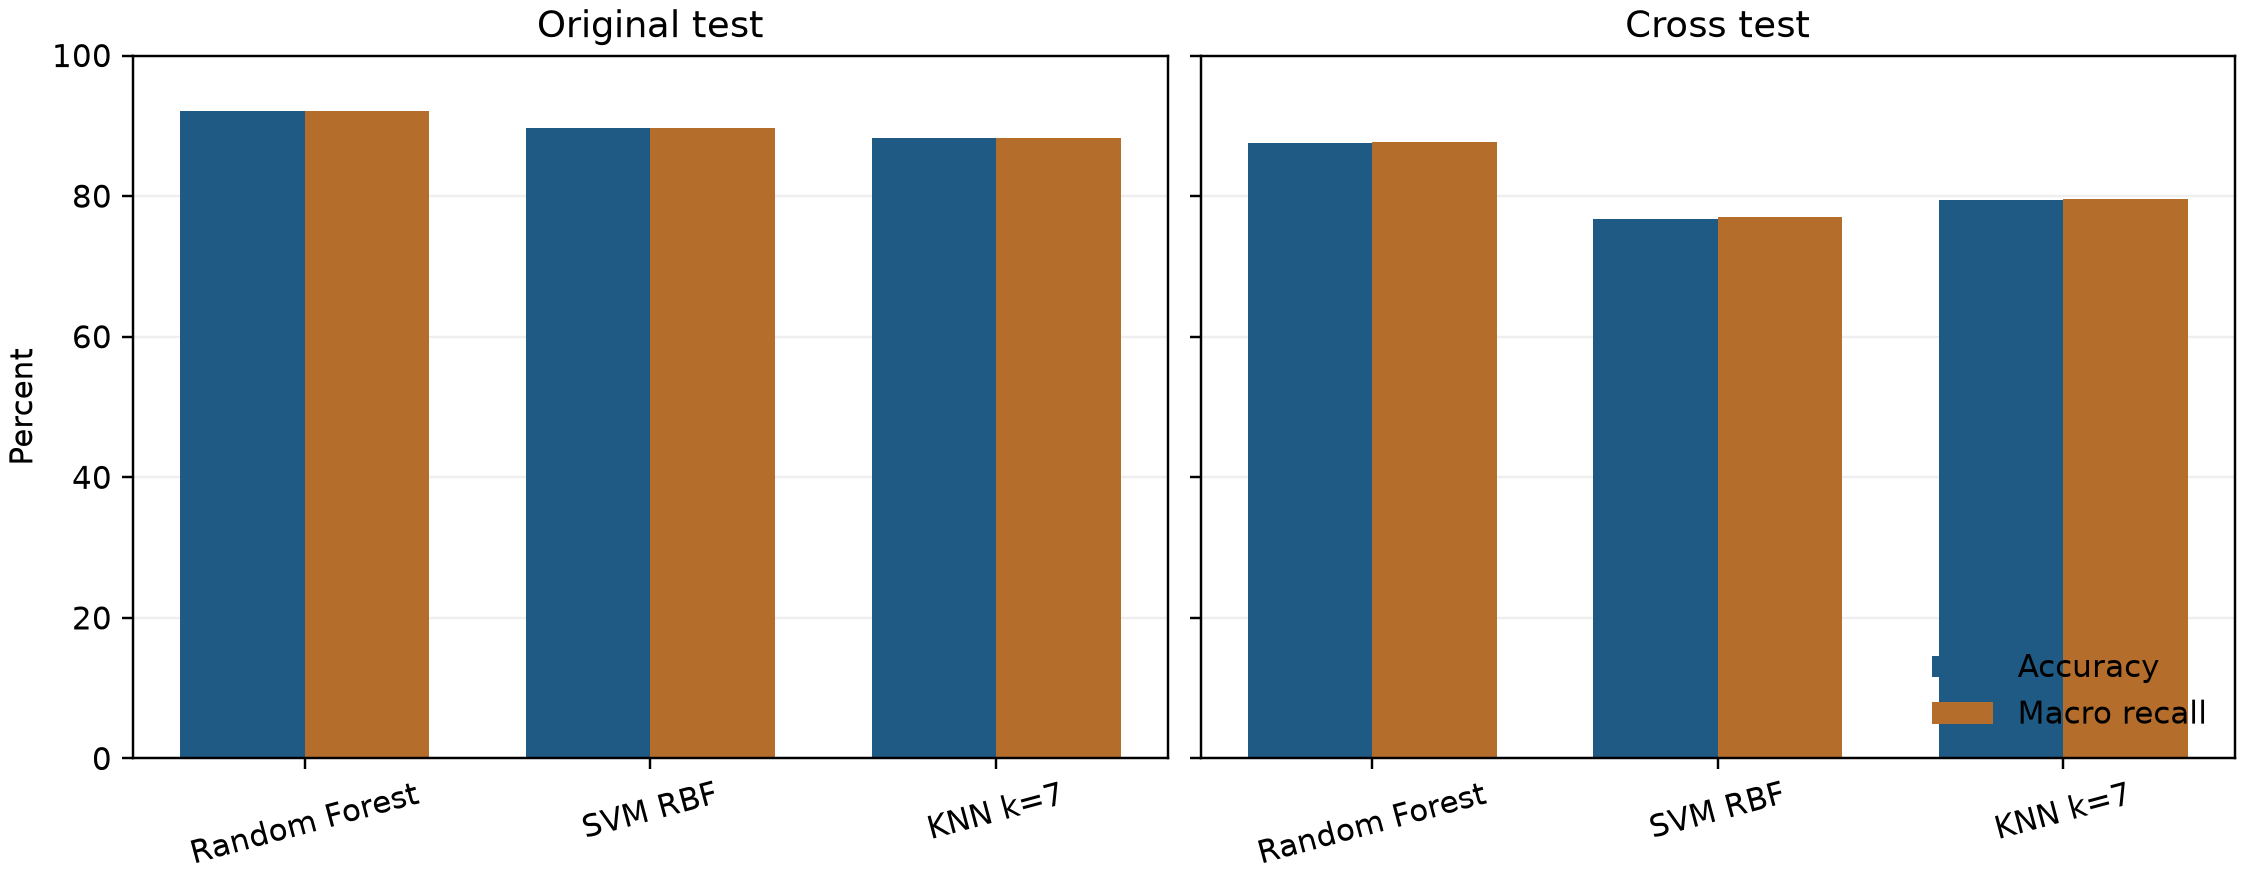
\includegraphics[width=\columnwidth]{accuracy_recall.png}
\caption{JA4Tor accuracy and macro recall.}
\label{fig:ja4tor}
\end{figure}

\subsection{MineShark Capture-Disjoint Evaluation}
\begin{table}[t]
\caption{MineShark capture-disjoint results (percent).}
\label{tab:mineshark}
\centering
\small
\begin{tabular}{lrrrrr}
\toprule
Model & Train & Test & Acc. & Recall & F1\\
\midrule
RF & 4743 & 1719 & 94.30 & 94.30 & 94.30\\
SVM & 4743 & 1719 & 97.27 & 97.27 & 97.27\\
KNN & 4743 & 1719 & 92.44 & 92.44 & 92.43\\
\bottomrule
\end{tabular}
\end{table}

SVM recalls for ShadowsocksR, Trojan, and VMess are 98.60\%, 96.51\%, and 96.68\%. Comparisons with JA4Tor must account for different labels, units, and workloads.
\subsection{Workload Shift}
When NBMiner captures are used for training and XMRig captures for testing, RF, SVM, and KNN obtain 44.81\%, 46.66\%, and 55.34\% accuracy, respectively. This experiment uses 3,702 training and 1,899 test windows. RF, SVM, and KNN macro F1 are 46.08\%, 42.87\%, and 54.55\%, respectively. SVM loses 50.61 percentage points relative to capture-disjoint evaluation. KNN superiority is limited to this fixed setting. This degradation indicates that workload and capture conditions can dominate the apparent decision boundary.
\begin{figure}[t]
\centering
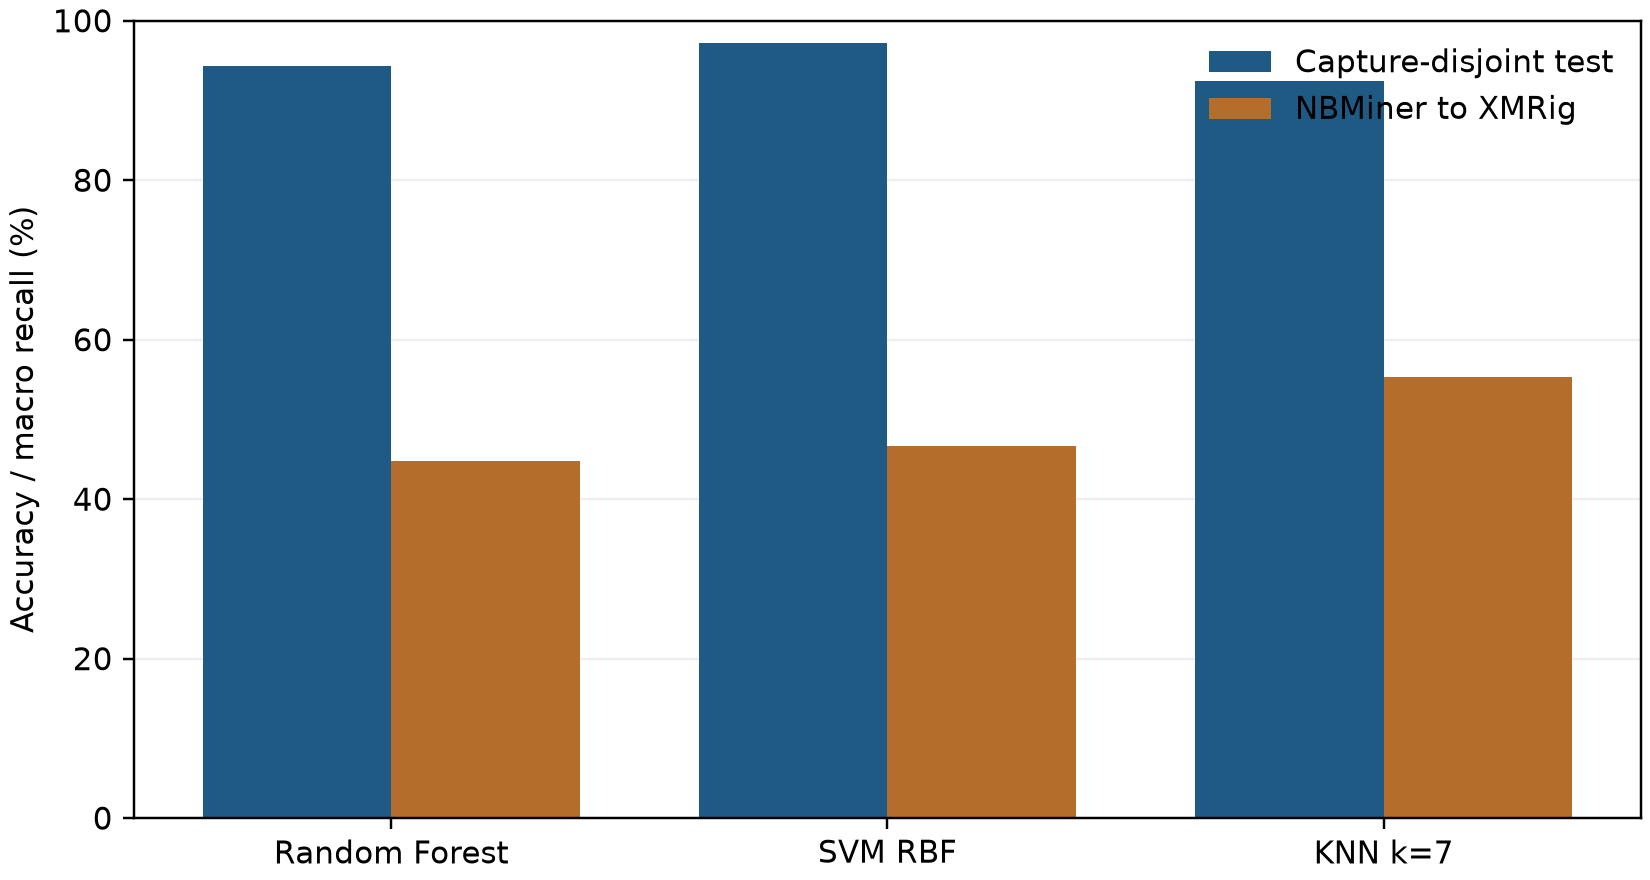
\includegraphics[width=\columnwidth]{workload_shift_comparison.png}
\caption{Workload-shift performance from NBMiner to XMRig.}
\label{fig:shift}
\end{figure}

\subsection{Feature Importance}
The RF mean-decrease-in-impurity ranking identifies the following leading features on JA4Tor: Bwd Packet Length Max (8.19\%), Fwd Packet Length Std (6.97\%), and Down/Up Ratio (6.79\%), followed by additional length and IAT statistics. These features describe directional burst size and asymmetry, giving an interpretable indication of what the classifier uses. The identical RF configuration was refitted on 20,000 training flows and reproduced 92.12\% test accuracy. The top ten account for 57.18\% of importance. MDI can favor continuous or high-cardinality variables, while correlated variables share importance; the ranking is neither causal nor guaranteed stable across networks.
\begin{figure}[t]
\centering
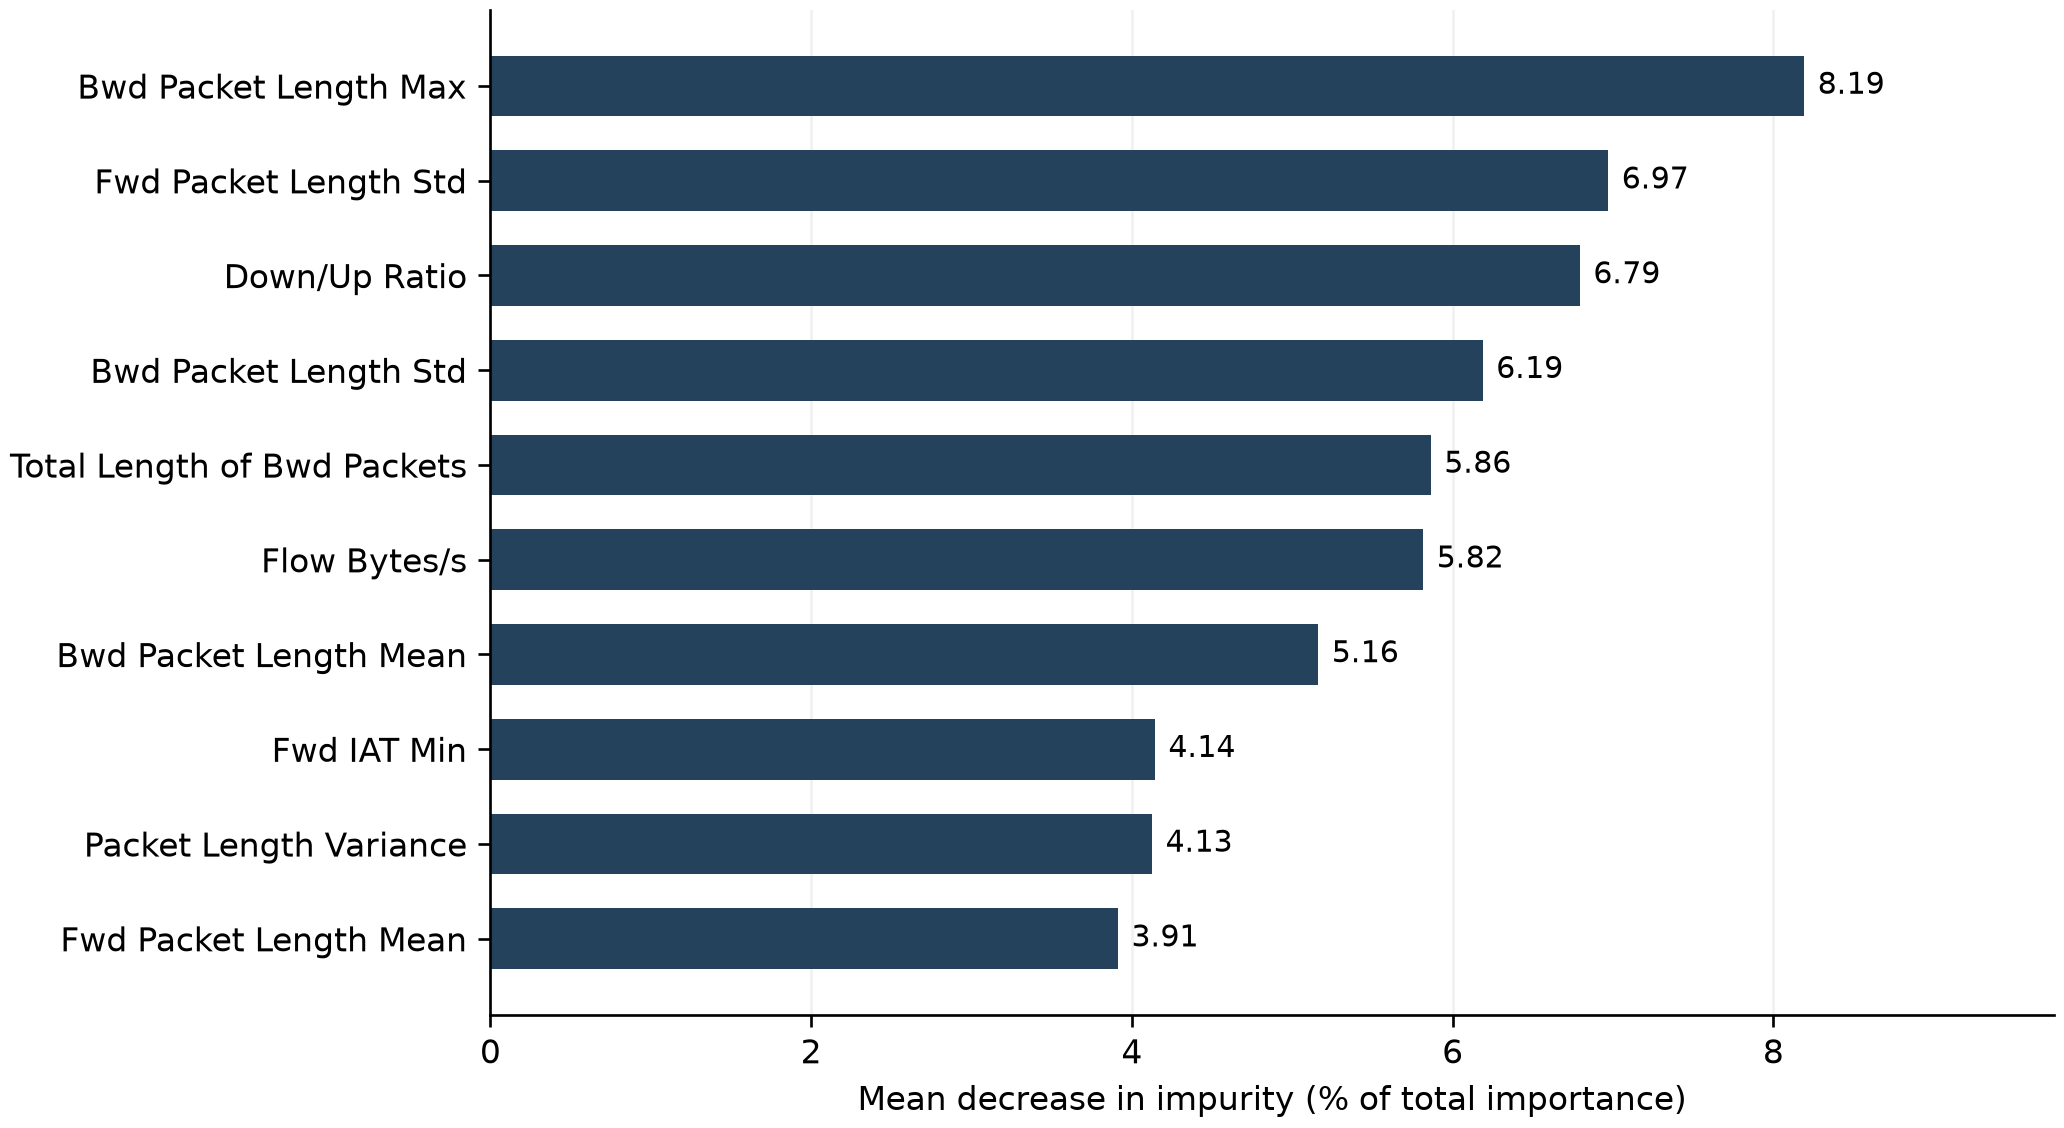
\includegraphics[width=\columnwidth]{feature_importance.png}
\caption{Top RF feature-importance ranking.}
\label{fig:importance}
\end{figure}

\section{Extended Results and Resource Costs}
Ten-repeat means, sample standard deviations, and nominal 95\% confidence intervals for JA4Tor and MineShark are computed from all ten saved runs. JA4Tor RF internal accuracy is 87.14\% (SD 0.45; CI [86.86,87.42]); MineShark capture-disjoint RF accuracy is 95.13\% (SD 2.21; CI [93.77,96.50]). Full summaries for six models and metrics are in results/extended/.

Every model's fixed-test per-class Precision, Recall, F1, and confusion matrices are exported under results/extended/. JA4Tor RF values are NonTor 99.80/99.60/99.70, Tor 99.69/95.30/97.44, Tor-SS 78.41/88.60/83.19, Tor-Trojan 99.79/93.40/96.49, and Tor-VMess 85.41/83.70/84.55 percent. MineShark seed-42 RF values are ShadowsocksR 99.44/96.62/98.01, Trojan 96.75/88.38/92.37, and VMess 88.73/98.92/93.55 percent. Full matrices are saved as CSV.

RF permutation importance ranks Fwd Packet Length Std (11.16 percentage-point mean accuracy decrease), Bwd Packet Length Max (1.76), Down/Up Ratio (1.22), Flow IAT Min (0.90), and Bwd Packet Length Std (0.90). Fixed-test RF trains in 2.27 s, predicts in 0.14 s, and serializes to 20.38 MB; SVM 8.98 s/5.54 s and 1.71 MB; KNN 0.17 s/0.42 s and 4.96 MB; Logistic Regression 4.21 s/0.01 s and 3.6 kB; HistGB 9.70 s/0.12 s and 1.28 MB; XGBoost 8.46 s/0.10 s and 1.77 MB. These are host-specific measurements.
\section{Discussion and Limitations}
The results support statistical flow classification as a useful baseline, but they also show why split design matters. A random row split can benefit from correlated flows from the same capture, while capture-disjoint and workload-shift tests are more demanding. The public sources do not provide complete and consistent labels for all proxy families requested in a four-class taxonomy. Consequently, the findings should be interpreted as benchmark-specific evidence rather than universal protocol identification.

Proxy and application behavior, network path, server, capture year, client implementation, and TLS transport can confound statistical fingerprints~\cite{xue}. Future four-class evaluation should use matched browsing tasks, multiple independent nodes and capture rounds, saved PCAP hashes and protocol configurations, and node/run-disjoint partitions. Unknown proxies and padding/multiplexing should also be tested.
\section{Conclusion}
We presented a reproducible pipeline for encrypted proxy traffic classification using 30 flow statistics and three classical classifiers. RF performs strongly on the original JA4Tor split, SVM performs best on the source-capture-disjoint three-class MineShark mining-trace split, and all methods degrade under workload shift. Feature ranking and explicit label auditing improve interpretability and prevent overclaiming.

\section{Code and Data Availability}
Scripts, result files, figures, metadata, and the editable paper source are available at:\newline
\url{https://github.com/silenceyuana/encrypted-proxy-traffic-identification}.

\section{Generative AI Usage Disclosure}
OpenAI Codex assisted with manuscript drafting, Chinese/English expression and polishing, experiment-code development, figure creation, and layout checking. Training, evaluation, and feature-importance values were computed by local Python/scikit-learn programs; AI-generated prose is not an experimental data source. The author is responsible for reviewing all text, references, code, and results before submission and for the final manuscript accuracy, originality, and research integrity.


\appendix
\section{Reproduction Instructions}
The recorded environment is Python 3.12, scikit-learn 1.9.1, and XGBoost 3.4.1. The complete experiment script and per-run result files are included in the repository. The repository scripts \texttt{run\_ja4tor\_baseline.py}, \texttt{run\_mineshark\_proxy\_baseline.py}, and \texttt{run\_mineshark\_workload\_shift.py} reproduce the three experiments. \texttt{plot\_workload\_shift.py} generates the comparison plot, and \texttt{analyze\_feature\_importance.py} regenerates feature rankings and the methodology figure. Run each with Python from the project root using the \texttt{scripts/} prefix. Experiment manifests and capture-split CSVs record versions, hashes, feature definitions, and partitions. Original third-party data are downloaded separately; raw archives are not redistributed. Data sources: \url{https://github.com/das-lab/JA4Tor} and \url{https://zenodo.org/records/13624058}.

\begin{thebibliography}{00}
\bibitem{gil} G. Draper-Gil et al., ``Characterization of encrypted and VPN traffic using time-related features,'' in \emph{Proc. ICISSP}, 2016, pp. 407--414. [Online]. Available: \url{https://www.unb.ca/cic/datasets/vpn.html}
\bibitem{xue} D. Xue et al., ``Fingerprinting obfuscated proxy traffic with encapsulated TLS handshakes,'' in \emph{Proc. 33rd USENIX Security Symp.}, 2024. [Online]. Available: \url{https://www.usenix.org/conference/usenixsecurity24/presentation/xue-fingerprinting}
\bibitem{nesttor} C. Zhou et al., ``NESTTOR: Detecting Tor-over-Proxy traffic with factorized decisions,'' \emph{IEEE Trans. Netw. Service Manag.}, 2026, doi: 10.1109/TNSM.2026.3743261.
\bibitem{mineshark} S. Xi et al., ``MineShark: Cryptomining traffic detection at scale,'' in \emph{Proc. NDSS}, 2025, doi: 10.14722/ndss.2025.230402.
\bibitem{breiman} L. Breiman, ``Random forests,'' \emph{Machine Learning}, vol. 45, pp. 5--32, 2001, doi: 10.1023/A:1010933404324.
\bibitem{cortes} C. Cortes and V. Vapnik, ``Support-vector networks,'' \emph{Machine Learning}, vol. 20, pp. 273--297, 1995, doi: 10.1007/BF00994018.
\bibitem{cover} T. Cover and P. Hart, ``Nearest neighbor pattern classification,'' \emph{IEEE Trans. Inf. Theory}, vol. 13, no. 1, pp. 21--27, 1967, doi: 10.1109/TIT.1967.1053964.
\bibitem{pedregosa} F. Pedregosa et al., ``Scikit-learn: Machine learning in Python,'' \emph{J. Mach. Learn. Res.}, vol. 12, pp. 2825--2830, 2011.
\end{thebibliography}
\end{document}








